% A section s of a sheaf F over an open set U, drawn as a curve above U.
% Source: book/tex/alg-geom/sheaves.tex (§ picturing sections).
\documentclass[border=2mm]{standalone}
\usepackage{tikz}
\usepackage{amssymb}
\begin{document}
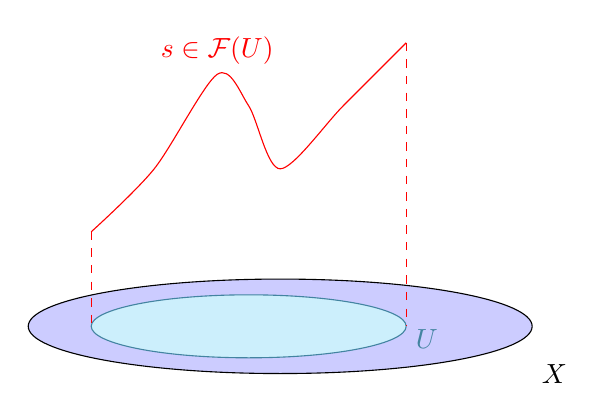
\begin{tikzpicture}[scale=0.4]
  \filldraw[blue!20, draw=black] (0,0) ellipse (8 and 1.5);
  \node at (8,-1.5) [right] {$X$};
  \filldraw[cyan!20, draw=cyan!60!black] (-1,0) ellipse (5 and 1);
  \node[cyan!60!black] at (4,-1) [above right] {$U$};
  \draw[red] plot[smooth] coordinates {(-6,3)(-4,5)(-2,8)(-1,7)(0,5)(2,7)(4,9)};
  \node[red] at (-2,8) [above] {$s \in \mathcal F(U)$};
  \draw[red,dashed] (-6,3) -- (-6,0);
  \draw[red,dashed] (4,9) -- (4,0);
\end{tikzpicture}
\end{document}
